\documentclass{standalone}
\usepackage{tikz}
\usepackage{amsmath}
\usepackage{color}

\usetikzlibrary{arrows.meta}
\usetikzlibrary{calc}
\usetikzlibrary{shapes}
\usetikzlibrary{bending}
\usetikzlibrary{patterns}

\usepackage{gensymb}


\begin{document}
	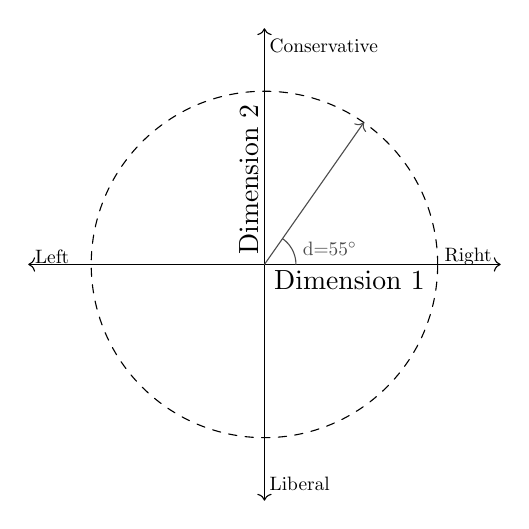
\begin{tikzpicture}[scale=2,cap=round]

\coordinate (c) at (2,0);
\draw[dashed] (c) circle (1.1cm);

\draw[->] (2.0,0)  -- (2.0,1.5) ;
\draw[->] (2.0,0)  -- (2.0,-1.5);
\draw[->] (2.0,0)  -- (0.5,0) ;
\draw[->] (2.0,0)  -- (3.5,0);   

\node[right, black] at (2.0,-0.1) {Dimension 1};
\node[right, black, rotate=90] at (1.9,0.0) {Dimension 2};

\node[right, black, scale=0.7] at (0.5,0.05) {Left};
\node[right, black, scale=0.7] at (3.1,0.05) {Right};

\node[right, black, scale=0.7] at (1.99,-1.39) {Liberal};
\node[right, black, scale=0.7] at (1.99,1.39) {Conservative};

\draw[->, black!70] (c) -- ($(c)+(55:1.1cm)$);
\draw[black!70,domain=0:55] plot ({2+0.2*cos(\x)}, {0.2*sin(\x)});

\node[right, black!70, scale=0.7] at (2.2,0.1) {d=55$\degree$};

%\coordinate (p1) at ($(c)+(15:1cm)$);
%\coordinate (p2) at ($(c)+(-15:1cm)$);
%\draw[dashed, black!50] (2.0,0)    -- (p1);
%\node[right, black, rotate=15] at (p1) {$15\degree$};
%\draw[dashed, black!50] (2.0,0)    -- (p2);  
%\node[right, black, rotate=-15] at (p2) {$345\degree$};

%\fill[fill=black!50] (p1) circle (1pt);
%\fill[fill=black!50] (p2) circle (1pt);
\end{tikzpicture}
\end{document}